\documentclass[11pt,a4paper]{article}

\usepackage[margin=2.5cm]{geometry}
\usepackage[T1]{fontenc}
\usepackage[utf8]{inputenc}
\usepackage{lmodern}
\usepackage{booktabs}
\usepackage{tabularx}
\usepackage{multirow}
\usepackage{graphicx}
\usepackage{xcolor}
\usepackage{amsmath}
\usepackage[numbers,sort&compress]{natbib}
\usepackage[hidelinks]{hyperref}

% Red placeholders for text that is still missing. Remove before submission.
\newcommand{\todo}[1]{\textcolor{red}{[TODO: #1]}}

\title{Steam Review Translator: Sentiment Distributions, Aspect Tables and Meta-Reviews
from Batches of Game Reviews}
\author{Muhammad Farrel Wibowo\\13523153\\Task 1
  \and Mahesa Fadhillah Andre\\13523140\\Task 2
  \and Lukas Raja Agripa\\13523158\\Task 3}
\date{IF5153 Advanced Natural Language Processing, Group 17}

\begin{document}
\maketitle

% =========================================================================================
\begin{abstract}
A popular game on Steam collects thousands of user reviews, far more than a buyer can read.
We present the Steam Review Translator, a pipeline that turns a batch of reviews of one game
into three outputs: (1) the distribution of positive, negative and neutral sentiment,
(2) a table of the aspects players discuss (gameplay, story, performance, \dots) with the
polarity expressed towards each, and (3) a short meta-review. For sentiment, a fine-tuned
RoBERTa classifier reaches a macro-F1 of 0.801 on Metacritic user reviews of unseen games and
0.846 on Steam reviews, and estimates per-game sentiment shares within 2.9 percentage points
(total variation distance). For aspects, we build a 7,002-sentence aspect-sentiment dataset
labeled by a large language model and train a LoRA-adapted RoBERTa tagger that reaches a
pair F1 of 0.586 and an aspect-detection F1 of 0.732 on held-out games, against 0.315 for a
lexicon baseline. For meta-reviews, we fine-tune BART on GameWikiSum with the aspect table as
an input prefix; it reaches a ROUGE-L of 0.180 against 0.109--0.121 for extractive and zero-shot
baselines, and the aspect prefix raises aspect coverage (0.340 to 0.379) without changing ROUGE.
The three components
share one typed interface and run end to end.
\end{abstract}

% =========================================================================================
\section{Introduction}

Steam reviews are the main signal buyers use to judge a game, but they arrive in volume:
the 2017 Steam review dump alone contains 6.4 million reviews over almost ten thousand games
\citep{sobkowicz2017steam}. The binary ``recommended'' flag compresses this into a single
percentage, which hides \emph{why} players like or dislike a game: a title may be praised for
its story and still be unplayable because of crashes.

We address this with a three-stage pipeline that ``translates'' a batch of reviews of one game
into information a buyer can read in seconds:
\begin{enumerate}
  \item \textbf{Task 1, sentiment distribution:} the share of positive, negative and neutral
    reviews, which refines the binary recommend flag with a neutral class.
  \item \textbf{Task 2, aspect table:} which aspects the reviews mention, how often, and with
    which polarity.
  \item \textbf{Task 3, meta-review:} a short natural-language summary of the reception,
    conditioned on the aspect table.
\end{enumerate}

Our contributions are: (i) a modular pipeline with a typed contract between the three tasks,
so each component can be swapped independently; (ii) a sentiment study that evaluates both
review-level accuracy and the per-game distribution, which is the quantity users actually see;
(iii) a 7,002-sentence aspect-sentiment dataset for Steam reviews, labeled with a large language
model under a written guideline, and a parameter-efficient tagger trained on it; and (iv) an
aspect-conditioned meta-review generator, together with the finding that the aspect prefix makes
the output follow the table more closely while ROUGE stays the same.

% =========================================================================================
\section{Related Work}

\paragraph{Sentiment analysis.} Lexicon-based methods such as VADER \citep{hutto2014vader}
need no training data but miss domain vocabulary; fine-tuned pretrained encoders such as
BERT \citep{devlin2019bert} and RoBERTa \citep{liu2019roberta} are the standard strong
baselines, and models trained on social media \citep{barbieri2020tweeteval} are often used
off the shelf.

\paragraph{Aspect-based sentiment analysis (ABSA).} ABSA identifies the aspects mentioned in
a text and the sentiment towards each \citep{pontiki2014semeval}. Topic models such as
BERTopic \citep{grootendorst2022bertopic} can discover aspect-like themes without labels.
Large language models have been shown to annotate text at or above crowd-worker quality
\citep{gilardi2023chatgpt}, which we use to build training data. LoRA \citep{hu2022lora} lets
us fine-tune an encoder on a laptop GPU by training a small number of parameters.

\paragraph{Opinion and meta-review summarization.} Opinion summarization condenses many
reviews into one text \citep{brazinskas2020copycat}. GameWikiSum
\citep{antognini2020gamewikisum} pairs game reviews with summaries from Wikipedia.
Extractive baselines such as TextRank \citep{mihalcea2004textrank} select sentences; abstractive
models such as BART \citep{lewis2020bart} and T5 \citep{raffel2020t5} generate new text.

% =========================================================================================
\section{System Overview}
\label{sec:system}

Figure~\ref{fig:pipeline} shows the pipeline. Its input is a game title and a list of reviews
(text plus the optional recommend flag); its output is a JSON object with the sentiment
distribution, the aspect table and the meta-review. Task~1 reads whole reviews. Task~2 splits
every review into sentences with one shared sentence splitter (spaCy), tags each sentence with
zero or more \emph{(aspect, polarity)} pairs, and aggregates them per game: the frequency of an
aspect is the number of sentences that mention it, and its polarity is the majority polarity of
those mentions (ties become neutral). Task~3 receives the reviews, the sentiment distribution and
the aspect table and generates the meta-review. Tasks~1 and~2 are independent.

All data passed between tasks follows one schema contract (pydantic models), and each task is
accessed only through a small interface (\texttt{SentimentAnalyzer.analyze},
\texttt{AspectTagger.tag}, \texttt{MetaReviewGenerator.generate}). A YAML file selects which
implementation each task uses, so every system in this paper, including the baselines, plugs
into the same pipeline.

\begin{figure}[t]
  \centering
  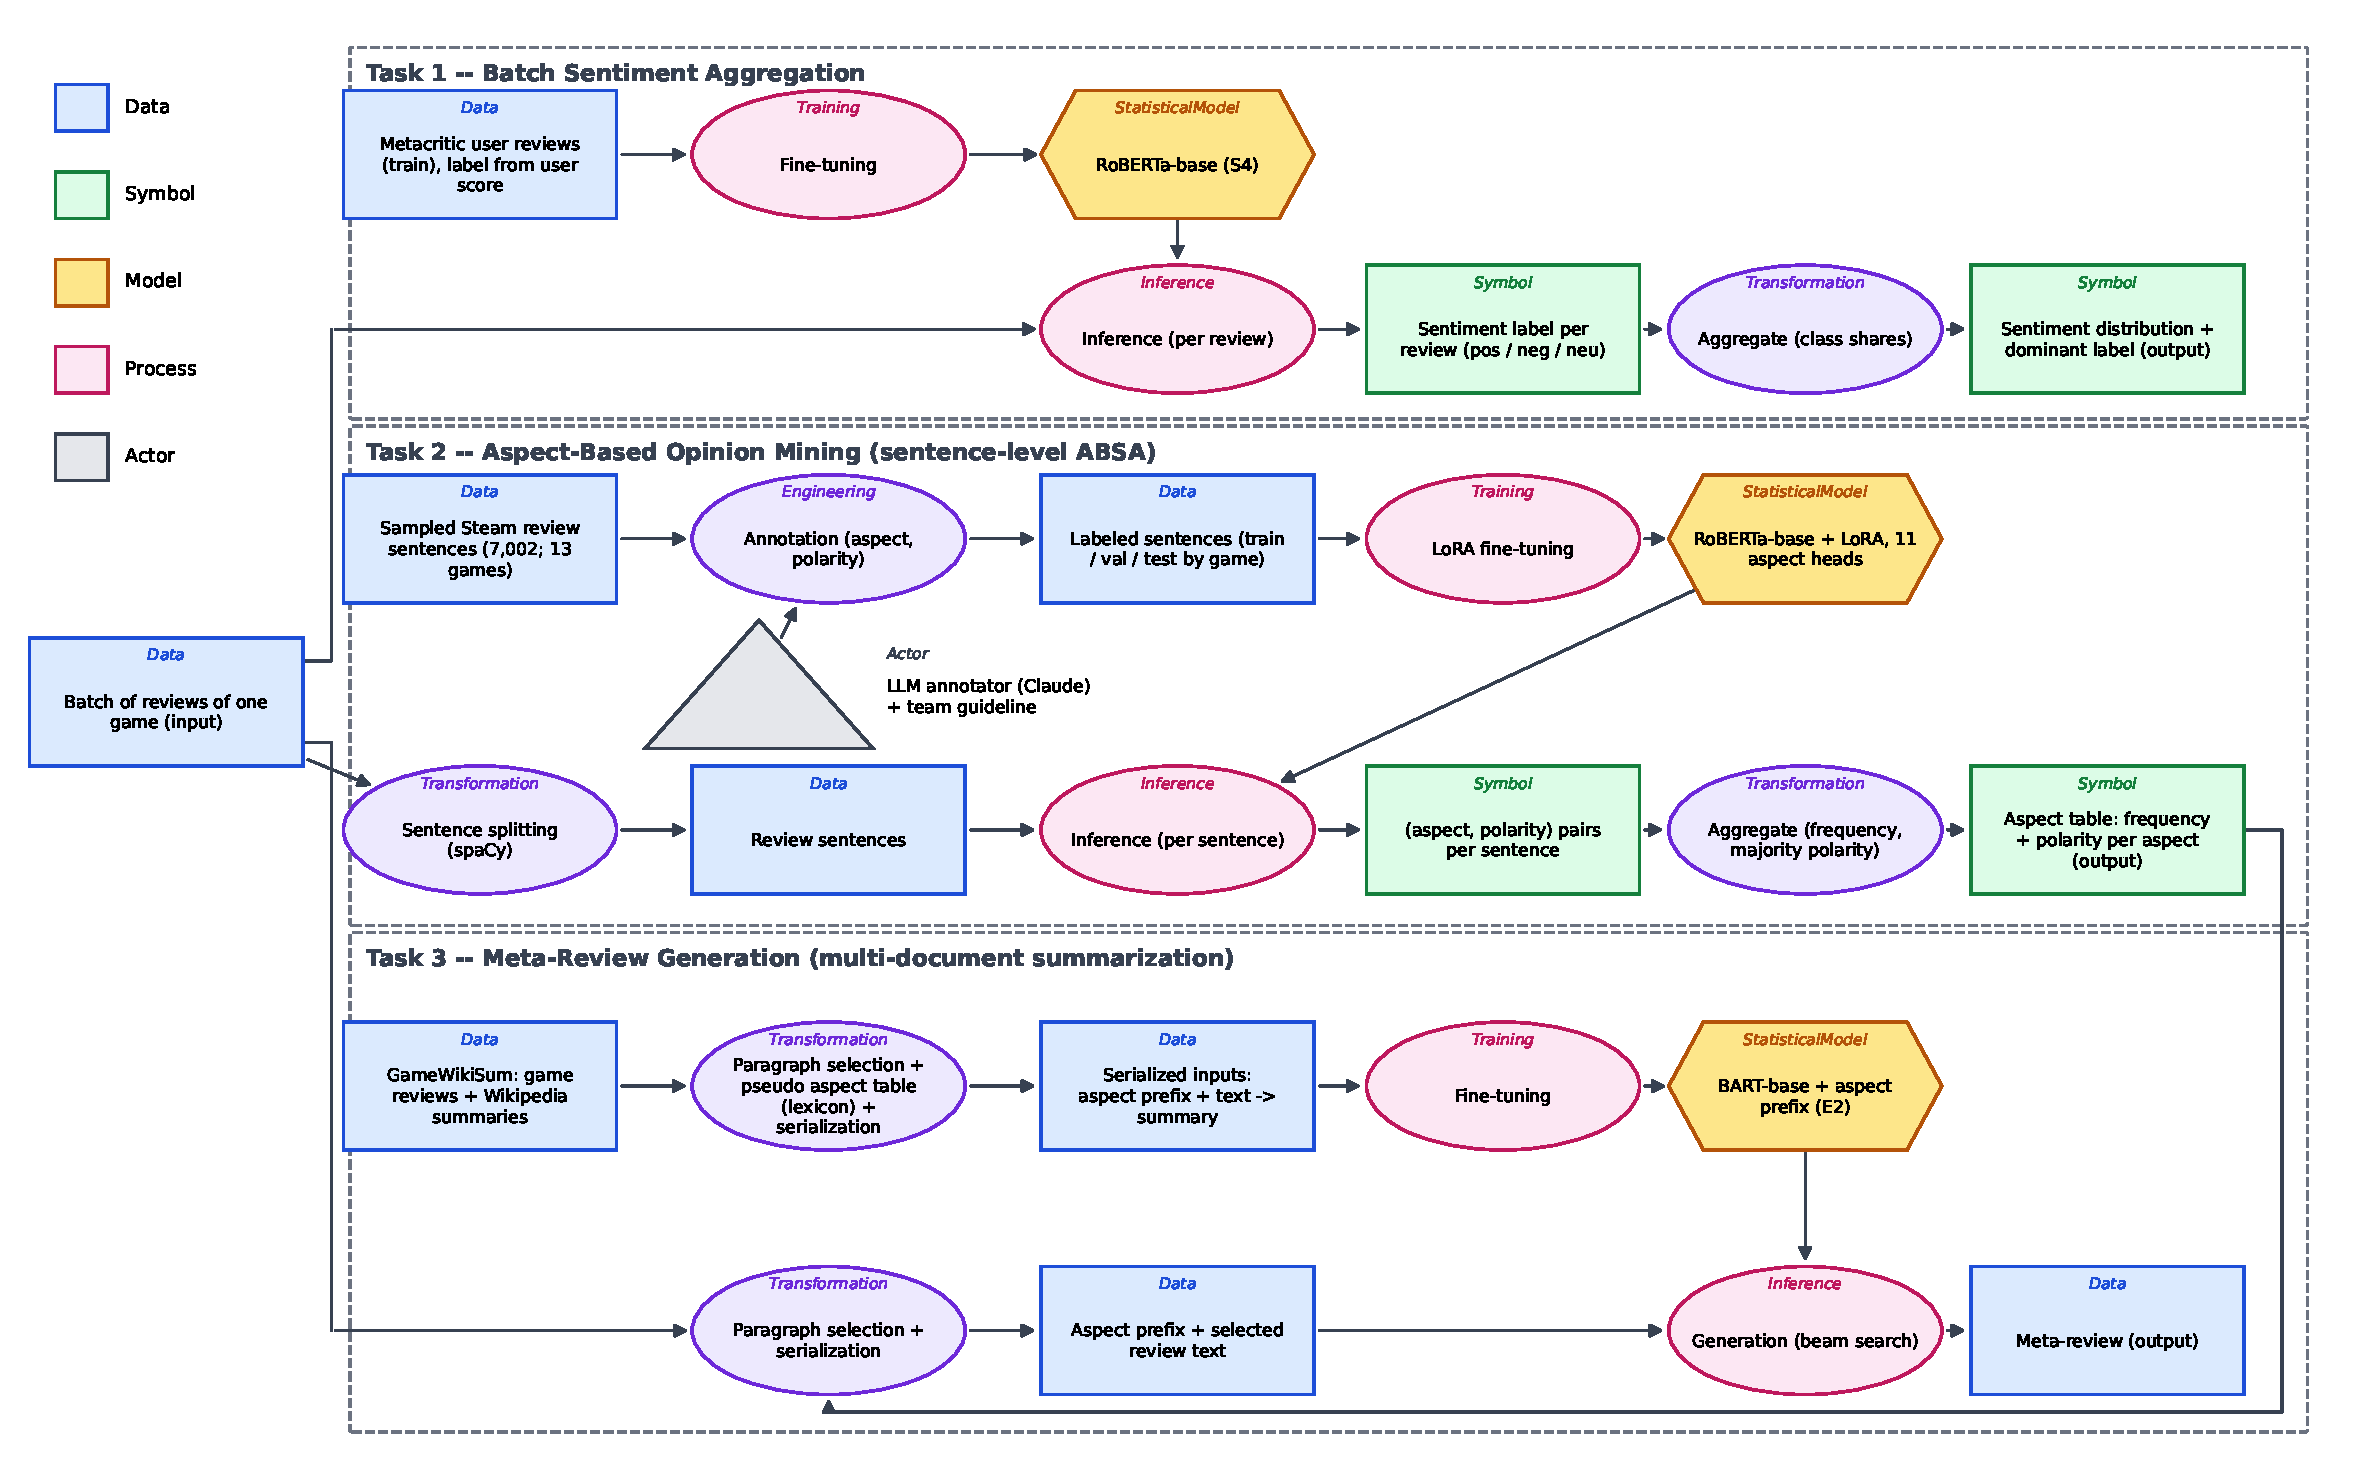
\includegraphics[width=\linewidth]{beam/beam_pipeline.pdf}
  \caption{The Steam Review Translator in BEAM notation. Blue boxes are data, green boxes symbols,
  purple hexagons statistical models, rounded boxes processes (orange: training, yellow: inference
  and transformation, red: engineering) and the triangle an actor. The batch of reviews is shared by
  the three tasks, and the aspect table produced by Task~2 is an input of Task~3. The
  machine-readable description is in \texttt{paper/beam/beam.ttl}.}
  \label{fig:pipeline}
\end{figure}

% =========================================================================================
\section{Task 1: Sentiment Distribution}
\label{sec:task1}

\subsection{Data}

\paragraph{Metacritic (train, validation, test).} We use the user reviews of the Kaggle
``Metacritic's Best Games and Reviews 2025'' dataset \citep{metacritic2025kaggle}. A review is
labeled from its 0--10 user score with Metacritic's colour bands: 0--4 negative, 5--7 neutral,
8--10 positive. We keep English reviews of at least three words, select 200 games that have at
least 300 usable reviews (stratified into five strata by the game's positive share, so mixed
and negative games are represented) and cap each game at 2,000 reviews. Games, not reviews, are
split 70/15/15 so test games are unseen. Table~\ref{tab:t1data} gives the statistics.

\paragraph{Steam (out-of-domain test).} 10,000 English reviews from 50 Steam apps (200 per
app, apps stratified by recommend share) from the Steam Review Dataset
\citep{sobkowicz2017steam}. Steam has only a binary recommend flag, so three-class predictions
are collapsed to binary by comparing the positive and negative scores. A manual check of 100
random Steam reviews, labeled from the text blind to the flag, found that 13\% of reviews are
neutral or mixed, and that the flag agrees with the text on 97.7\% of polar reviews.

\begin{table}[t]
  \centering
  \small
  \begin{tabular}{lrrrr}
    \toprule
    & Train & Val & Test & Steam \\
    \midrule
    Games & 140 & 30 & 30 & 50 \\
    Reviews & 124,837 & 25,743 & 24,257 & 10,000 \\
    Labels & \multicolumn{3}{c}{pos 58.8\% / neg 27.7\% / neu 13.5\% (all)} & binary \\
    \bottomrule
  \end{tabular}
  \caption{Task 1 data. Metacritic is split by game.}
  \label{tab:t1data}
\end{table}

\paragraph{Training examples} (Metacritic train split, text as written by users).
\emph{Resident Evil 5}, score 10 $\rightarrow$ positive: ``My cousin and I had a lot of fun
playing this game back in the day \dots\ Lots of replay value and quite the adventure.''
\emph{FIFA 21}, score 0 $\rightarrow$ negative: ``Unrealistic, extremely borring and broken. Its
not about winning or losing, I dont enjoy this game even when I win.''
\emph{Watch Dogs: Legion}, score 6 $\rightarrow$ neutral: ``Meh. Its mediocre at best, I loved
the past 2 games and this just felt really bland. Like, it isn't bad, but its just so
middling.''

\subsection{Models}

\begin{itemize}
  \item \textbf{S0, VADER} \citep{hutto2014vader}: rule-based compound score, threshold
    $\pm0.05$.
  \item \textbf{S1, TF-IDF + logistic regression}: word uni- or bi-grams (sublinear TF,
    min.\ document frequency 3, at most 300k features), class-balanced logistic regression;
    $C\in\{0.25,1,4\}$ and the n-gram range are chosen on validation.
  \item \textbf{S2, zero-shot}: the pretrained three-class
    \texttt{twitter-roberta-base-sentiment-latest} model \citep{barbieri2020tweeteval},
    without further training.
  \item \textbf{S3, BERT} and \textbf{S4, RoBERTa}: \texttt{bert-base-uncased}
    \citep{devlin2019bert} and \texttt{roberta-base} \citep{liu2019roberta} fine-tuned for
    three-class classification.
\end{itemize}

\subsection{Experimental setting}

S3 and S4 are fine-tuned for three epochs with AdamW (learning rate $2\times10^{-5}$, weight
decay 0.01, 6\% linear warm-up), batch size 32, inputs truncated to 256 tokens and mixed
precision on one T4 GPU (Google Colab). The checkpoint with the best validation macro-F1
(evaluated every 2,000 steps) is kept: 0.813 for S4 and 0.796 for S3. Each system is run once
on the test sets.

We report review-level accuracy and macro-F1, and distribution-level errors per game, which is
what the pipeline outputs: the mean absolute error (MAE) and total variation distance (TVD)
between the predicted and the gold class shares, and the share of games whose dominant class
is predicted correctly.

\subsection{Results}

\begin{table}[t]
  \centering
  \small
  \begin{tabular}{lcccccccc}
    \toprule
    & \multicolumn{2}{c}{Metacritic test} & \multicolumn{2}{c}{Steam} &
      \multicolumn{3}{c}{Metacritic per game} \\
    \cmidrule(lr){2-3}\cmidrule(lr){4-5}\cmidrule(lr){6-8}
    System & Acc & Macro-F1 & Acc & Macro-F1 & MAE & TVD & Dominant \\
    \midrule
    S0 VADER & 0.709 & 0.484 & 0.802 & 0.661 & 0.120 & 0.181 & 0.73 \\
    S1 TF-IDF + LR & 0.819 & 0.733 & 0.832 & 0.776 & 0.038 & 0.057 & 0.97 \\
    S2 zero-shot & 0.787 & 0.587 & 0.843 & 0.783 & 0.073 & 0.109 & 1.00 \\
    S3 BERT & 0.862 & 0.783 & 0.885 & 0.835 & 0.023 & 0.035 & 1.00 \\
    S4 RoBERTa & \textbf{0.877} & \textbf{0.801} & \textbf{0.892} & \textbf{0.846} &
      \textbf{0.019} & \textbf{0.029} & 0.97 \\
    \bottomrule
  \end{tabular}
  \caption{Task 1 test results. Per-game errors are computed over the 30 Metacritic test
  games; Dominant = share of games whose most frequent class is predicted correctly.}
  \label{tab:t1results}
\end{table}

Table~\ref{tab:t1results} shows that the fine-tuned encoders are clearly best: S4 reaches a
macro-F1 of 0.801 on unseen Metacritic games and 0.846 on Steam, and its per-game sentiment
shares are off by 1.9 percentage points on average. VADER almost never predicts neutral
(F1 0.041) and over-predicts positive by 14 points per game. On Steam the ranking holds,
although the learned systems (S1--S4) under-estimate the positive share per game by 7--12
points.

\subsection{Error analysis}

\paragraph{Neutral is the hard class.} S4's F1 is 0.943 for positive and 0.856 for negative
but 0.604 for neutral. Accuracy falls at the label boundaries of the user score: 0.917 at
score~0 and 0.974 at score~10, but 0.653 at~4, 0.555 at~5, 0.674 at~7 and 0.741 at~8. These
reviews are genuinely ambiguous, because the label comes from a number the text does not
always reflect: a training review of \emph{S.T.A.L.K.E.R.~2} scored 6 (neutral) reads ``the
game is raw, lots of bugs, bad shooting \dots\ so many years of development to get this
crap.''

\paragraph{Long reviews.} The model sees at most 256 tokens; accuracy drops from 0.896 for
reviews under 25 words to 0.784 for reviews over 400 words on Metacritic.

\paragraph{Steam and the binary flag.} 11.2\% of all Steam reviews are recommended but
predicted neutral; collapsing to binary recovers most of them (76\% correct). Against labels
read from the text, S4 is correct on 96.6\% of polar reviews, so part of the remaining Steam
error is label noise in the flag (sarcasm, recommendations despite complaints about price).

% =========================================================================================
\section{Task 2: Aspect Table}
\label{sec:task2}

\subsection{Task definition}

Each sentence receives zero or more \emph{(aspect, polarity)} pairs. The aspects are
\emph{gameplay, story, graphics, audio, performance, price, multiplayer, difficulty} and
\emph{content}, plus \emph{overall} for verdicts on the whole game and \emph{other} for
opinions outside these classes; polarity is positive, negative or neutral; a sentence with no
opinion gets no label. At most one label per aspect is allowed in a sentence.

\subsection{Data and labeling}

\paragraph{Source and sample.} From the Steam Review Dataset \citep{sobkowicz2017steam}
(6,417,106 reviews; 4,817,044 clean English reviews after language identification and
quality filtering) we selected 13 games and split them \emph{by game} into 9 training,
2 validation and 2 test games. We sampled 75 reviews per game (975 reviews) and split them into
7,002 sentences (Table~\ref{tab:t2data}).

\paragraph{LLM labeling.} Labeling 7,002 sentences by hand was not feasible within the project,
so we labeled them with Claude Opus \citep{anthropic2025claude} under a written guideline that
defines each aspect with examples and edge cases (e.g.\ always-online requirements count as
\emph{performance}, not \emph{multiplayer}). The model reads each review in full and labels its
sentences one by one. For the first 22 of 63 batches (2,422 sentences, including the whole test
split), a second model (Claude Sonnet, and Opus for the first 14 batches) reviewed every label
and a third pass decided the flagged sentences. Review changed only 10 of 2,422 labels (0.4\%),
so the remaining batches were labeled by Opus alone. A local 7B open model (Qwen2.5) was also
tried as a cheaper labeler but agreed poorly with Opus (pair F1 0.55--0.62), so it was not
used. The labels are silver labels: they measure agreement with the LLM, not with people.

\begin{table}[t]
  \centering
  \small
  \begin{tabular}{lrrrrrr}
    \toprule
    Split & Games & Reviews & Sentences & No aspect & Labels/sent. & Words/sent. \\
    \midrule
    Train & 9 & 675 & 5,150 & 15.0\% & 1.05 & 14.5 \\
    Val & 2 & 150 & 1,001 & 12.0\% & 1.11 & 15.4 \\
    Test & 2 & 150 & 851 & 14.7\% & 1.08 & 13.8 \\
    \midrule
    All & 13 & 975 & 7,002 & 14.5\% & 1.06 & 14.6 \\
    \bottomrule
  \end{tabular}

  \vspace{0.6em}
  \begin{tabular}{lrrrr|lrrrr}
    \toprule
    Aspect & Sent. & Pos & Neg & Neu & Aspect & Sent. & Pos & Neg & Neu \\
    \midrule
    gameplay & 1,802 & 31\% & 51\% & 18\% & story & 505 & 34\% & 42\% & 24\% \\
    overall & 1,620 & 57\% & 36\% & 7\% & other & 431 & 16\% & 75\% & 8\% \\
    performance & 823 & 9\% & 84\% & 6\% & price & 351 & 26\% & 59\% & 15\% \\
    graphics & 534 & 58\% & 30\% & 11\% & multiplayer & 344 & 24\% & 65\% & 12\% \\
    content & 516 & 33\% & 54\% & 13\% & difficulty & 310 & 25\% & 42\% & 34\% \\
    & & & & & audio & 219 & 53\% & 40\% & 8\% \\
    \bottomrule
  \end{tabular}
  \caption{Task 2 dataset: split statistics (top) and label distribution over all splits
  (bottom). Test games: \emph{Sniper: Ghost Warrior 2} and \emph{Two Worlds II HD};
  validation: \emph{Might \& Magic: Heroes VI} and \emph{Paper Sorcerer}.}
  \label{tab:t2data}
\end{table}

\paragraph{Training examples.} ``There are a few downsides, animations could have been better
and the combat felt a little janky.'' $\rightarrow$ graphics/negative, gameplay/negative.
``My favorite RTS, i still havent gotten around to playing campaign.'' $\rightarrow$
overall/positive. ``Go slow and always have a fresh clip.'' $\rightarrow$ no label.

\subsection{Systems}

\begin{itemize}
  \item \textbf{Seed lexicon (baseline).} A hand-written keyword list per aspect; every aspect
    found in a sentence gets the sentence's polarity from a small list of positive and negative
    words.
  \item \textbf{System A, induced lexicon + VADER.} The seed lexicon is extended with 681
    unigrams and bigrams induced from the \emph{training} labels: a term is added to an aspect
    if at least five training sentences containing it carry that aspect and they make up at
    least half of the sentences containing it (thresholds tuned on validation). Polarity is the
    sentence's VADER score.
  \item \textbf{System C, LoRA-tuned RoBERTa.} \texttt{roberta-base} with LoRA adapters
    \citep{hu2022lora} (rank 16, $\alpha=32$, dropout 0.1) on the attention query and value
    projections; the mean-pooled sentence encoding feeds one four-way classifier per aspect
    (\emph{not mentioned}, positive, negative, neutral). An aspect is predicted when
    $1-P(\textit{not mentioned})$ reaches a threshold; its polarity is the most likely polarity
    class. 623,660 parameters are trained.
\end{itemize}

A BERTopic-based system (topics mapped to aspects) was explored during data analysis but not
completed.

\subsection{Experimental setting}

System C is trained on the 5,150 training sentences with cross-entropy over all aspect heads,
AdamW (learning rate $3\times10^{-4}$, weight decay 0.01, 6\% warm-up), batch size 16, inputs of
at most 96 tokens, for 10 epochs (about 30\,s per epoch on a laptop RTX 4050). The epoch and the
threshold ($\{0.20, 0.25, \dots, 0.50\}$) are chosen by validation pair F1: epoch 9 and 0.45
(validation pair F1 0.621). Test is used once per system.

Metrics are computed per sentence: \emph{pair} precision, recall and F1 count an
(aspect, polarity) pair as correct only if both match; \emph{aspect} F1 ignores polarity;
\emph{polarity accuracy} is measured on aspects found by both gold and prediction; \emph{exact
match} is the share of sentences whose label set is exactly right.

\subsection{Results}

\begin{table}[t]
  \centering
  \small
  \begin{tabular}{lccccccc}
    \toprule
    System & Pair P & Pair R & Pair F1 & Aspect F1 & Macro F1 & Pol.\ acc & Exact \\
    \midrule
    Seed lexicon & 0.289 & 0.110 & 0.159 & 0.410 & 0.473 & 0.388 & 0.209 \\
    A: induced lexicon + VADER & 0.314 & 0.316 & 0.315 & 0.545 & 0.552 & 0.578 & 0.219 \\
    C: RoBERTa + LoRA & \textbf{0.613} & \textbf{0.561} & \textbf{0.586} & \textbf{0.732} &
      \textbf{0.714} & \textbf{0.801} & \textbf{0.474} \\
    \bottomrule
  \end{tabular}
  \caption{Task 2 test results (851 sentences, two unseen games). Macro F1 = macro-averaged
  aspect-detection F1.}
  \label{tab:t2results}
\end{table}

Table~\ref{tab:t2results} shows that System C nearly doubles the pair F1 of the lexicon system
(0.586 vs 0.315). Inducing terms from the training labels already doubles the seed lexicon,
but sentence-level VADER polarity remains its weak point (0.578 accuracy). Per aspect, System C
reaches an F1 of 0.90 for graphics, 0.83 story, 0.82 price, 0.80 audio, 0.76 overall,
0.73 gameplay, 0.71 performance, 0.67 multiplayer, 0.66 content, 0.64 difficulty and 0.35 for
other. Scores are similar on the two test games (pair F1 0.592 and 0.580).

\subsection{Error analysis}

52.6\% of test sentences contain at least one error. Missed aspects are the most common error
(259 sentences), followed by extra aspects (183) and wrong polarity (123); 108 sentences with
an aspect receive no label at all.

\paragraph{Overall vs gameplay.} Most misses are \emph{overall} (70) and \emph{gameplay} (66),
often confused with each other: ``It's just too dull and boring.'' is an overall verdict in
the gold labels but tagged gameplay.

\paragraph{Missing context.} The tagger sees one sentence, while the labeler read the whole
review. Fragments such as ``Should stick with what works.'' or ``and were programed by a class
of kindergardeners\dots'' cannot be resolved without context.

\paragraph{Neutral polarity and \emph{other}.} Only 28 of 87 neutral aspect mentions are
predicted neutral, and \emph{other}, a heterogeneous class, is mostly missed (recall 0.23).

% =========================================================================================
\section{Task 3: Meta-Review Generation}
\label{sec:task3}

\subsection{Data}

GameWikiSum \citep{antognini2020gamewikisum} pairs the professional reviews of a game with a
section of its Wikipedia article. One sample is one game: the input is the paragraphs of all
its reviews and the target is the Wikipedia text, which in practice mostly describes the
gameplay (e.g.\ ``cat quest is an action role-playing video game played from a top-down
perspective \dots''). We use the official splits (Table~\ref{tab:t3data}). Inputs are very long
(about 11,000--12,000 words per game over the first 400 paragraphs) compared with the
1,024-token model input, which is why paragraph selection is needed.

\begin{table}[t]
  \centering
  \small
  \begin{tabular}{lrrrrr}
    \toprule
    Split & Documents & Games & Paragraphs/doc & Input words/doc & Summary words (mean / median) \\
    \midrule
    Train & 11,744 & 7,006 & 162.8 & 10,800 & 459.4 / 318 \\
    Val & 1,454 & 880 & 184.3 & 12,208 & 431.4 / 310 \\
    Test & 1,454 & 862 & 183.6 & 12,289 & 464.8 / 314 \\
    \bottomrule
  \end{tabular}
  \caption{GameWikiSum statistics. Paragraph and word counts use at most the first 400 review
  paragraphs of a document.}
  \label{tab:t3data}
\end{table}

\paragraph{Training example.} Game \emph{Hybrid}. Model input after preprocessing:
\texttt{aspects: multiplayer (9, neutral) ; gameplay (6, neutral) ; price (3, neutral) ;
content (2, neutral) ; performance (1, neutral) </s>} ``hybrid is a unique experiment in
multiplayer cover-based shooting, and it succeeds gloriously. the action is frantic and
non-stop \dots''. Target: ``players choose between the variant faction and the paladin faction
when they begin playing \dots''.

\subsection{Method}

The input is prepared in three steps.
\textbf{[A] Paragraph selection:} boilerplate and very short paragraphs are removed, the rest
are scored by TF-IDF relevance combined with aspect-lexicon matches ($\alpha=0.6$), and the
best are kept up to 800 tokens; documents with fewer than 100 words after cleaning are dropped.
\textbf{[B] Aspect table:} at training time a pseudo aspect table is computed from the selected
text with the Task~2 lexicon and a lexicon polarity rule; at inference time it is replaced by
the real Task~2 table. \textbf{[C] Serialization:} the five most frequent aspects are written as
a prefix, e.g.\ \texttt{aspects: gameplay (23, positive) ; graphics (12, negative) </s>}
followed by the text.

\begin{itemize}
  \item \textbf{B1}: extractive TextRank \citep{mihalcea2004textrank}, three sentences.
  \item \textbf{B2}: \texttt{bart-large-cnn} \citep{lewis2020bart} zero-shot.
  \item \textbf{E1}: \texttt{bart-base} fine-tuned on the text only.
  \item \textbf{E2}: \texttt{bart-base} fine-tuned with the aspect prefix (main system).
\end{itemize}
A T5-base variant with the aspect prefix (E3, \citealp{raffel2020t5}) was implemented but not
run within the time budget.

\subsection{Experimental setting}

E1 and E2 are fine-tuned on a pilot subset of 2,000 training documents for three epochs with
AdamW (learning rate $3\times10^{-5}$), effective batch size 32 (4 $\times$ 8 gradient
accumulation), mixed precision, at most 1,024 input and 256 target tokens, on one T4 GPU
(Google Colab; about 45 minutes per model). After every epoch, ROUGE-L is computed on 200
validation documents and the best epoch is kept. Decoding uses beam search (4 beams, no repeated
trigrams). All systems are evaluated once on the first 500 test documents (499 remain after
dropping documents with fewer than 100 words). We report ROUGE-1/2/L \citep{lin2004rouge}, the
share of the table's top aspects that the output mentions (aspect coverage), polarity
consistency with the table, and a paired bootstrap test (1,000 resamples) for E2 vs E1.

\subsection{Results}

\begin{table}[t]
  \centering
  \small
  \begin{tabular}{lccccc}
    \toprule
    System & ROUGE-1 & ROUGE-2 & ROUGE-L & Aspect cov. & Pol.\ cons. \\
    \midrule
    B1 TextRank & 0.177 & 0.028 & 0.109 & 0.291 & 0.596 \\
    B2 BART-large-CNN zero-shot & 0.193 & 0.030 & 0.121 & \textbf{0.385} & 0.655 \\
    E1 BART-base, text only & 0.311 & \textbf{0.077} & \textbf{0.180} & 0.340 & 0.954 \\
    E2 BART-base + aspects & \textbf{0.320} & \textbf{0.077} & \textbf{0.180} & 0.379 &
      \textbf{0.964} \\
    \bottomrule
  \end{tabular}
  \caption{Task 3 test results on GameWikiSum (499 documents). E2 vs E1 ROUGE-L: mean
  difference $-0.0001$, 95\% CI $[-0.0024, 0.0020]$, $p=0.91$ (paired bootstrap).}
  \label{tab:t3results}
\end{table}

Fine-tuning matters most: E1 and E2 reach a ROUGE-L of 0.180, against 0.109 for TextRank and
0.121 for zero-shot BART-large-CNN, which was trained on news and copies review sentences rather
than describing the game. The aspect prefix does not change ROUGE (E2 vs E1: ROUGE-L difference
$-0.0001$, $p=0.91$), but it moves the output towards the aspects in the table: aspect coverage
rises from 0.340 to 0.379 and polarity consistency from 0.954 to 0.964. On validation, ROUGE-L
was flat across epochs (0.175--0.179 for E2), so more training data rather than more epochs is
the likely way to improve.

\subsection{Error analysis}

We classified 50 test outputs per system, stratified by ROUGE-L, into hallucination,
repetition, missed aspect or wrong polarity, Wikipedia-style description instead of opinion,
and input failure (Table~\ref{tab:t3errors}).

\begin{table}[t]
  \centering
  \small
  \begin{tabular}{lccccc}
    \toprule
    System & Hallucination & Missed aspect & Descriptive style & Other errors & No error \\
    \midrule
    B2 zero-shot & 40 & 0 & 8 & 0 & 2 \\
    E1 & 0 & 2 & 45 & 0 & 3 \\
    E2 & 1 & 0 & 48 & 0 & 1 \\
    \bottomrule
  \end{tabular}
  \caption{Error categories on 50 test outputs per system (automatic heuristics; other errors
  are repetition and input failure, none observed).}
  \label{tab:t3errors}
\end{table}

\paragraph{The target is description, not opinion.} Almost every fine-tuned output is a
Wikipedia-style description of how the game is played, because that is what the references
are. The fine-tuned models learned this style well (best E2 output, \emph{Cat Quest},
ROUGE-L 0.311: ``cat quest is an action role-playing game played from a third-person
perspective \dots'') but the result is a game description rather than a summary of what
reviewers think. This is a mismatch between GameWikiSum and our meta-review goal.

\paragraph{Generic and invented content.} Low-scoring outputs drift into generic genre text
or wrong entities, e.g.\ for \emph{Anito: Defend a Land Enraged} (ROUGE-L 0.047) E2 starts with
``super mario bros is an action role-playing game \dots''. B2 mostly copies or recombines review
sentences, which the heuristic counts as hallucination (40 of 50).

% =========================================================================================
\section{End-to-End Example}
\label{sec:demo}

We ran the pipeline on 200 random reviews of \emph{Two Worlds II HD}, a Task~2 test game
(54.5\% of the reviews recommend it). The aspect table from System C ranks gameplay (297
sentences, positive) and overall (287, positive) first, followed by performance (92,
negative), graphics (86, positive), story (77, positive), content (74, positive) and price (71,
negative), which matches the common complaints about this game's technical state and price.
This run used the models available on one machine: for Task~1 the zero-shot S2 model (which
predicts 45\% positive, 47\% negative and 8\% neutral, and so gets the dominant label wrong)
and for Task~3 the zero-shot B2 generator, which returned a copy of one positive review
(``Two Worlds II has a classless, fluid gameplay that allows you to be what you want to
be \dots''). The fine-tuned S4 and E2 weights are stored outside the repository; by the
results in Sections~\ref{sec:task1} and~\ref{sec:task3}, S4 would correct the sentiment shares
and E2 would produce a game description conditioned on the aspect table.

% =========================================================================================
\section{Limitations}

\begin{itemize}
  \item \textbf{Silver labels.} Task~2 gold labels come from an LLM and were not verified by
    people before evaluation; Task~1 labels come from user scores or the recommend flag, which
    do not always match the text.
  \item \textbf{Sentence-only aspect tagging.} The Task~2 tagger sees one sentence without the
    rest of the review, which causes many of its errors.
  \item \textbf{Small aspect test set.} Task~2 is tested on two games (851 sentences); rare
    aspects (multiplayer has 4 validation sentences) make validation choices noisy.
  \item \textbf{Training/inference mismatch in Task~3.} The generator is trained with pseudo
    aspect tables from a lexicon but receives the Task~2 model's tables in the pipeline; and
    GameWikiSum differs from our target setting (its inputs are not Steam user reviews and its
    references are Wikipedia text, not opinion summaries).
  \item \textbf{Small Task~3 budget.} E1 and E2 were trained on 2,000 of 11,744 training
    documents and evaluated on 500 of 1,454 test documents; T5 (E3) was not run.
  \item \textbf{Limited search.} One seed per model and little hyperparameter search.
\end{itemize}

% =========================================================================================
\section{Conclusion}

We built a pipeline that turns a batch of Steam reviews into a sentiment distribution, an
aspect table and a meta-review. Fine-tuned encoders give accurate per-game sentiment shares,
and a LoRA-tuned RoBERTa trained on LLM-labeled sentences clearly outperforms lexicon methods
for aspect tagging. For meta-reviews, fine-tuning BART on GameWikiSum clearly beats extractive
and zero-shot baselines, and the aspect prefix steers the output towards the table, but the
references teach a descriptive style rather than an opinion summary. Future work: give the
aspect tagger review context, verify a subset of the aspect labels by hand, and train the
meta-review generator on opinion-style references and real aspect tables.

\paragraph{Code and data.} Code: \url{https://github.com/mahesa005/steam-review-translator}.
The Task~2 aspect dataset (7,002 labeled sentences) is in the repository
(\texttt{data/processed/task2\_labels.jsonl.gz}), together with the trained System~C adapter.
Task~1 data are rebuilt from the original Metacritic (Kaggle) and Steam (Zenodo) sources with
our preparation scripts, and Task~3 uses GameWikiSum from its authors (academic use only, not
redistributed) through our loading and preprocessing code.

\bibliographystyle{plainnat}
\bibliography{references}

\end{document}
